\subsection{Validation} \label{sec:validation}

As an optional task the LWC13 task requires the implementation of
analysis rules. Xtext provides a validation framework which integrates into the
EMF Validation
framework\footnote{\url{http://www.eclipse.org/modeling/emf/?project=validation}}.
The Xtext User Manual contains a Validation chapter that is
worth reading additionally\footnote{see
\url{http://www.eclipse.org/Xtext/documentation.html\#validation}}.

We will show in this section how the constraints defined in the task description
can be realized with Xtext.

\subsubsection{Extending the Java Validator class}
With the first translation of the Xtext grammar, the generator has already
created the necessary infrastructure to implement custom validation rules.
Look into the package \texttt{org.eclipse.xtext.example.ql.validation}, you will
find a Java class \texttt{QlDslJavaValidator}. The class extends the
\texttt{AbstractQlDslJavaValidator} class, which is regenerated each time the
grammar is translated. Thus, the generation gap pattern is applied here again.
It is safe to extend the \texttt{QlDslJavaValidator} class manually.

But instead of implementing the constraints in Java, we will use Xtend again.
For easier integration, our Xtend based validator class will be inserted into
the class hierarchy of QlDslJavaValidator.

Create an Xtend class \texttt{QlDslXtendValidator}, and extend it from
\texttt{AbstractQlDslJavaValidator}.

\begin{lstlisting}[language=Xtend]
package org.eclipse.xtext.example.ql.validation

import javax.inject.Inject
import org.eclipse.xtext.validation.Check
import org.eclipse.xtext.xbase.XFeatureCall
import org.eclipse.xtext.xbase.XbasePackage
import org.eclipse.xtext.xbase.jvmmodel.IJvmModelAssociations

import static extension org.eclipse.xtext.nodemodel.util.NodeModelUtils.*
class QlDslXtendValidator extends AbstractQlDslJavaValidator {
  @Inject extension IJvmModelAssociations
}
\end{lstlisting}

Derive QlDslJavaValidator from the the Xtend validator:

\begin{lstlisting}[language=Java]
public class QlDslJavaValidator extends QlDslXtendValidator {
  // do nothing here, rules are implemented in Xtend
}
\end{lstlisting}

\subsubsection{Constraint: Ensure order of questions}

The first constraint in the LWC13 task is defined so:

\begin{quote}
\emph{
Test for cyclic dependencies. For instance, the following snippet should be rejected:
}
\begin{lstlisting}[language=QL]
if (x) { y: "Y?" boolean }
if (y) { x: "X?" boolean }
\end{lstlisting}

\emph{The reason is that y will only be asked for when x is true, but x will only get a value when y is true. 
Of course such cyclic dependencies could occur transitively and nested in expressions. 
Another way of stating this check is: the ordering of questions should be
consistent with how the question variables are used in conditions and computed values. 
}
\end{quote}

The task allows two approaches to achieve the goal. We will choose the second
approach: Check that elements referred in expressions have been declared before
their usage.

Xtext does not enforce that elements are declared before they are used
somewhere. The referred names simply must be in the scope of the context, which
the current scope implementation already accomplishes. We could implement this
constraint also in the scope provider of the language by restricting the scope
to elements that have been declared before. However, we will implement this as a
semantic constraint in the validator class.

To implement the constraint we need to know the location in the model where a
Question element is declared and where it is called in an expression. Besides
the Abstract Syntax Tree Xtext maintains a second model, which represents the
document. This is the so-called \emph{Node Model}, and the class
\texttt{NodeModelUtils} provides some utility functions to navigate from an AST
element to the node model. Since Questions that are referred in expressions are
local to the Form, we can simply compare the offset in the document of the
declared Question and the feature call in an expression.

Xtext validation rules are implemented as methods which are annotated with
\texttt{@Check}. The method name does not matter. Check methods are expected to
have exactly one parameter, which is of the type of element that has to be
checked. The base class provides methods to create error messages. For the case
of this constraint, the necessary context object type is \texttt{XFeatureCall}. 

Now open the \texttt{QlDslXtendValidator} class again and add this
method\footnote{\url{https://gist.github.com/kthoms/5240455}}:

\begin{lstlisting}[language=Xtend]
  @Check
  def void check_featureDeclaredBeforeCall (XFeatureCall featureCall) {
    val featureSource = featureCall.feature.sourceElements.head
    val nodeFeature = if (featureSource != null) featureSource.node else featureCall.feature.node
    val nodeCall = featureCall.node
    if (nodeFeature != null) {
      if (nodeFeature.offset > nodeCall.offset) {
        error(featureCall.feature.simpleName+" must be declared before.",featureCall, 
        XbasePackage::eINSTANCE.XAbstractFeatureCall_Feature, "ERR_FEATURE_CALL_BEFORE_DECLARATION", null)
      }
    }
  }
\end{lstlisting}

After restarting the workbench the situation will be recognized as an error:

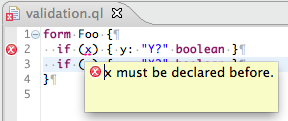
\includegraphics[width=6cm]{images/chapter04/validation_1.png}

\subsubsection{Constraint: Type conformance check}

Next, the LWC13 task requires checking the type conformance in expressions:

\begin{quote}
\emph{Type check conditions and variables: the expressions in conditions should be
type correct and should ultimately be booleans. The assigned variables should be
assigned consistently: each assignment should use the same type.
}\end{quote}

Here we have to do nothing, since this constraint is already implemented in
Xbase. This works thanks to Xbase's type inference mechanism. The Xtend language
makes heavy use of this nice feature, which makes it almost unneccessary to
declare types anywhere. For dynamic languages this is natural, since the actual
type is known and evaluated at runtime. Static typed language often lack this
feature.

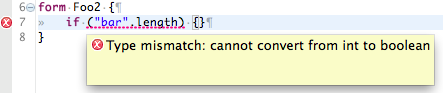
\includegraphics[width=6cm]{images/chapter04/validation_2.png}

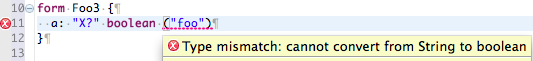
\includegraphics[width=6cm]{images/chapter04/validation_3.png}


\subsubsection{Testing validation rules}

It is easy to test validation rules in a runtime environment. However, we will
show how these rules can also be unit tested. Also herefore the Xtext framework
already contains the necessary infrastructure. Remember that Xtext has already
created a test plugin with the initial generator run? Now it is time to make use
of it.

Again, it is easier to create the test with Xtend. Xtend allows us to create
simple models inline with Rich Strings, pass the result to a parser, and
validate the result. With Xtend this is a one-liner.

\begin{lstlisting}[language=Xtend]
package org.eclipse.xtext.example.ql.validation.test

import javax.inject.Inject
import org.eclipse.xtext.example.ql.QlDslInjectorProvider
import org.eclipse.xtext.example.ql.qlDsl.Questionnaire
import org.eclipse.xtext.junit4.InjectWith
import org.eclipse.xtext.junit4.XtextRunner
import org.eclipse.xtext.junit4.util.ParseHelper
import org.eclipse.xtext.junit4.validation.ValidationTestHelper
import org.eclipse.xtext.xbase.XbasePackage
import org.junit.Before
import org.junit.Test
import org.junit.runner.RunWith

@RunWith(typeof(XtextRunner))
@InjectWith(typeof(QlDslInjectorProvider))
class QlDslValidationTest {
  @Inject extension ParseHelper<Questionnaire> parseHelper
  @Inject extension ValidationTestHelper
  
  @Before
  def void setUp () {
    parseHelper.fileExtension="ql"
  }
  
  @Test
  def void testValidation_CallBeforeDeclaration_expectError () {
    '''
    form Foo {
      if (x) { y: "Y?" boolean }
      if (y) { x: "X?" boolean }
    }
    '''.parse.assertError(XbasePackage::eINSTANCE.XFeatureCall, "ERR_FEATURE_CALL_BEFORE_DECLARATION", "must be declared before")
  }

  @Test
  def void testValidation_CallBeforeDeclaration_expectSuccess () {
    '''
    form Foo {
      x: "foo" boolean
      if (x) { a: "X?" boolean }
    }
    '''.parse.assertNoErrors
  }
  
  
  // Type check conditions and variables: the expressions in conditions should be type correct and should ultimately be booleans. 
  // The assigned variables should be assigned consistently: each assignment should use the same type.  
  @Test
  def void testValidation_ConditionTypeCheck_expectError () {
    '''
    form Foo {
      if ("foo".length) { a: "X?" boolean }
    }
    '''.parse.assertError(XbasePackage::eINSTANCE.XMemberFeatureCall, 
       "org.eclipse.xtext.xbase.validation.IssueCodes.incompatible_types", "Type mismatch")
  }
  
  @Test
  def void testValidation_ConditionTypeCheck_expectSuccess () {
    '''
    form Foo {
      if ("foo".length>1) { a: "X?" boolean }
    }
    '''.parse.assertNoErrors
  }

  @Test
  def void testValidation_AssignmentTypeCheck_expectFailure () {
    '''
    form Foo {
      a: "X?" boolean ("foo".length)
    }
    '''.parse.assertError(XbasePackage::eINSTANCE.XMemberFeatureCall, 
       "org.eclipse.xtext.xbase.validation.IssueCodes.incompatible_types", "Type mismatch")
  }

  @Test
  def void testValidation_AssignmentTypeCheck_expectSuccess () {
    '''
    form Foo {
      a: "X?" boolean ("foo".length>1)
    }
    '''.parse.assertNoErrors
  }
}
\end{lstlisting}

Basically, the class is a plain JUnit 4 class. We have to use a special
JUnit execution class, \texttt{XtextRunner}, and provide a language specific initializer
class, \texttt{QlDslInjectorProvider}.

Next, the class adds two extension classes. ParseHelper provides a parse()
method for char sequences. This will parse and validate the model. Afterwards
the observed issues can be asserted with the methods from the 

\begin{lstlisting}[language=Xtend]
@RunWith(typeof(XtextRunner))
@InjectWith(typeof(QlDslInjectorProvider))
class QlDslValidationTest { 
  @Inject extension ParseHelper<Questionnaire> parseHelper
  @Inject extension ValidationTestHelper
  ...
}
\end{lstlisting}

Now the test methods can be implemented. They are super simple:

\begin{lstlisting}[language=Xtend]
  @Test
  def void testValidation_CallBeforeDeclaration_expectSuccess () {
    '''
    form Foo {
      x: "foo" boolean
      if (x) { a: "X?" boolean }
    }
    '''.parse.assertNoErrors
  }
\end{lstlisting}
  
Due to the tight Java integration, the unit tests of the Xtend class can be
executed by running them through the context menu (\emph{Run As / JUnit Test}).

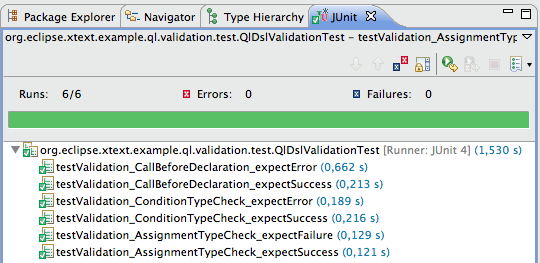
\includegraphics[width=12cm]{images/chapter04/validation_4.png}

